% =============================================================
% Capitulo 5 -- Resultados
% Padroes: ABNT, terceira pessoa, sem vicios de IA, sem listas
% \citeonline; \textit{F.\,catus} apos primeira mencao;
% legendas curtas+longas; \fonte; re-ID expandido na primeira mencao
% =============================================================

\chapter{Resultados}
\label{cap:resultados}

Este capítulo apresenta o conjunto de medidas obtidas com a execução do pipeline da Felinet sobre os dois corpora considerados, com foco no comportamento observado nas Fases II e III (detecção e classificação operacional) e na Fase IV (reidentificação, re-ID). A leitura privilegia a articulação entre o número observado, o desenho experimental descrito no Capítulo~\ref{cap:metodologia} e as decisões arquiteturais documentadas no Capítulo~\ref{cap:pipeline}. A discussão integrada de limitações e implicações, bem como o detalhamento de trabalhos futuros, é deslocada para o Capítulo~\ref{cap:conclusao}, conforme o recorte editorial adotado.

% -------------------------------------------------------------
\section{Ambiente de execução}
\label{sec:res-ambiente}

Todas as medidas reportadas neste capítulo foram coletadas em uma única estação de trabalho, com ambiente registrado de forma reprodutível por meio do utilitário \texttt{registrar\_ambiente.py}, cujo manifesto acompanha cada run no diretório \texttt{artifacts/}. As especificações relevantes para a interpretação dos tempos absolutos e da disponibilidade de aceleração por GPU encontram-se reunidas na Tabela~\ref{tab:cap5-ambiente}.

\begin{table}[!htb]
  \centering
  \caption[Ambiente de execução utilizado nos experimentos.]{Especificações do ambiente de execução utilizado em todos os runs reportados no Capítulo~\ref{cap:resultados}.}
  \label{tab:cap5-ambiente}
  \begin{tabular}{ll}
    \toprule
    \textbf{Componente} & \textbf{Valor registrado} \\
    \midrule
    Hostname            & felipi-pc \\
    Sistema operacional & Linux 6.8.0-117 (x86\_64), glibc 2.39 \\
    Interpretador       & Python 3.12.3 \\
    Aprendizado profundo & PyTorch 2.5.1 (CUDA 12.1) \\
    GPU                 & NVIDIA GeForce MX250 \\
    CUDA disponível     & sim \\
    Detector            & MegaDetector v5 (wrapper local) \\
    Classificador       & SpeciesNet (wrapper local) \\
    Backbone re-ID      & MegaDescriptor (extração de embeddings) \\
    \bottomrule
  \end{tabular}
  \fonte{Elaborado pelo autor a partir do manifesto \texttt{manifest.json} gerado por \texttt{registrar\_ambiente.py}.}
\end{table}

A combinação de uma GPU de notebook (MX250) com pacotes recentes de CUDA mostrou-se suficiente para inferência sequencial dos modelos selecionados sobre subconjuntos de até 300 imagens por fonte, conforme atestam os tempos absolutos discutidos na Seção~\ref{sec:res-cascata}. Não houve treinamento de modelos no estudo: tanto MegaDetector quanto SpeciesNet operaram em modo de inferência com pesos públicos, e MegaDescriptor produziu embeddings de 768~dimensões usados pelos protocolos closed-set e open-set descritos no Capítulo~\ref{cap:metodologia}.

% -------------------------------------------------------------
\section{Fases II e III: cascata operacional sobre fontes externas}
\label{sec:res-cascata}

A execução conjunta das Fases II (detecção por MegaDetector) e III (classificação por SpeciesNet) sobre dois subconjuntos de 300 imagens permitiu observar o comportamento da cascata em condições contrastantes. O corpus \texttt{kaggle\_cats} \cite{cat_dataset_kaggle_2024} reúne fotografias domésticas de \textit{Felis catus} em variedade de cenários, enquanto o corpus Felidae \cite{felidae_dataset_gts} agrupa imagens de felídeos não-domésticos, oriundas de cativeiro e de ambientes naturais. O contraste entre os dois é particularmente útil porque sustenta uma leitura simultânea de sensibilidade (capacidade de aceitar gatos domésticos) e de especificidade (capacidade de rejeitar outros felídeos da família Felidae).

Os volumes agregados por fonte estão sumarizados na Tabela~\ref{tab:cap5-fontes-resumo}, e os totais por fase, com as respectivas taxas derivadas, compõem a Tabela~\ref{tab:cap5-comparativo-fontes}. A representação visual conjunta dos dois conjuntos de dados aparece na Figura~\ref{fig:cap5-comparativo-fontes}.

\begin{table}[!htb]
  \centering
  \caption[Resumo das fontes operacionais ingeridas.]{Resumo das fontes operacionais ingeridas (volume, deduplicação por SHA-256, janela temporal e extensões observadas).}
  \label{tab:cap5-fontes-resumo}
  \begin{tabular}{lcccc}
    \toprule
    \textbf{Fonte} & \textbf{Mídias} & \textbf{Únicas (SHA-256)} & \textbf{Janela temporal} & \textbf{Extensões} \\
    \midrule
    \texttt{kaggle\_cats} & 300 & 300 & sem EXIF & .jpg (100\%) \\
    Felidae               & 300 & 300 & 2020--2025 & .jpg (100\%) \\
    \bottomrule
  \end{tabular}
  \fonte{Elaborado pelo autor a partir dos manifests de ingestão.}
\end{table}

\begin{table}[!htb]
  \centering
  \caption[Comparativo entre fontes na cascata Fases II e III.]{Comparativo entre as duas fontes operacionais nas Fases II e III: total ingerido, detecções de animais, classificações de \textit{F.\,catus} e taxas derivadas. Métricas extraídas dos runs mais recentes de cada fase.}
  \label{tab:cap5-comparativo-fontes}
  \begin{tabular}{lrrrrrr}
    \toprule
    \textbf{Fonte} & \textbf{Mídias} & \textbf{Detecções} & \textbf{Imgs c/ animal} & \textbf{Taxa animal} & \textbf{Class.\ \textit{F.\,catus}} & \textbf{Taxa \textit{F.\,catus}} \\
    \midrule
    \texttt{kaggle\_cats} & 300 & 308 & 184 & 61,3\% & 257 & 83,4\% \\
    Felidae               & 300 & 385 & 292 & 97,3\% & 1   & 0,3\% \\
    \bottomrule
  \end{tabular}
  \fonte{Elaborado pelo autor a partir dos artefatos \texttt{comparativo\_fontes.csv} (run \texttt{dm\_v8}).}
\end{table}

\begin{figure}[!htb]
  \centering
  \caption[Cascata operacional: volumes e taxas por fonte.]{Cascata operacional para os corpora \texttt{kaggle\_cats} e Felidae. O painel (a) reporta volumes absolutos por fase; o painel (b), as taxas relativas de detecção animal e de aceitação como \textit{F.\,catus}.}
  \label{fig:cap5-comparativo-fontes}
  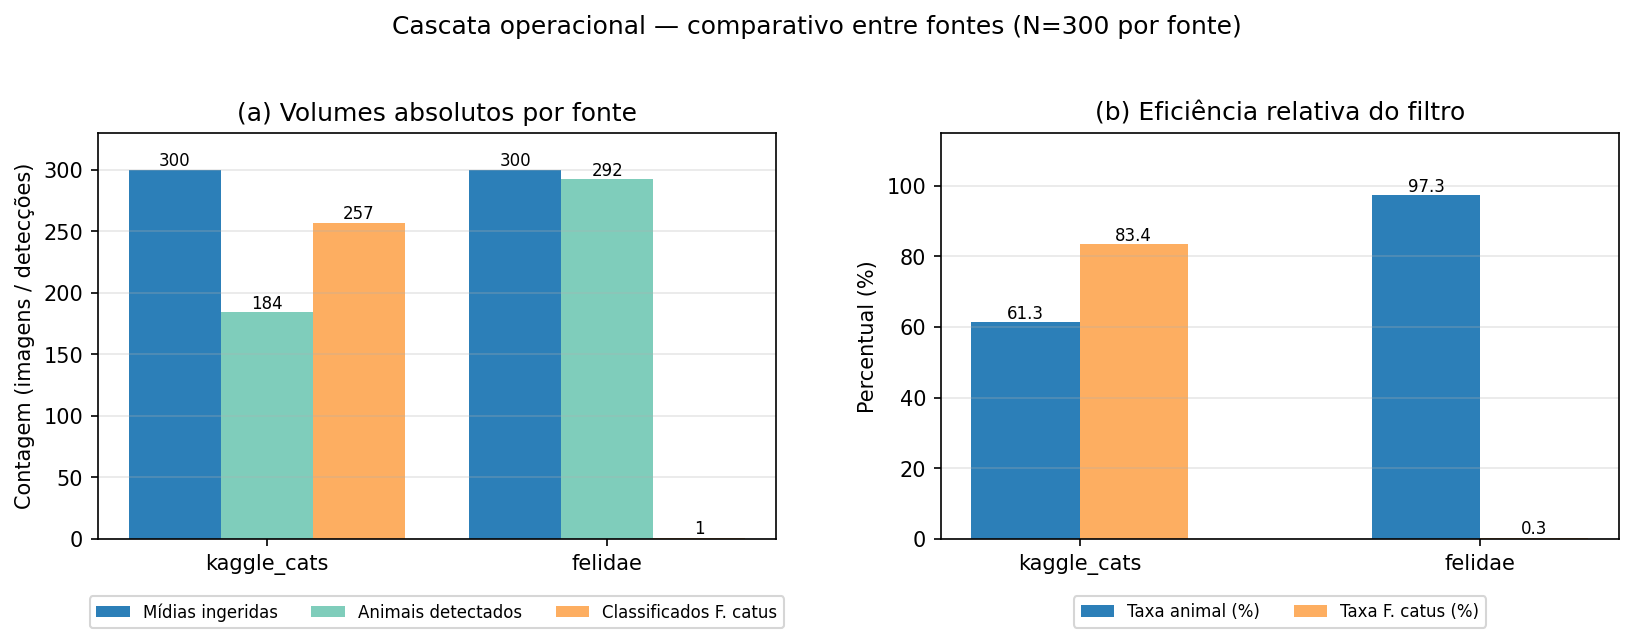
\includegraphics[width=0.95\linewidth]{elementos/figuras/cap5/comparativo_fontes_v8.png}
  \fonte{Elaborado pelo autor a partir dos artefatos da run \texttt{dm\_v8}.}
\end{figure}

A leitura conjunta da Tabela~\ref{tab:cap5-comparativo-fontes} e da Figura~\ref{fig:cap5-comparativo-fontes} expõe um padrão coerente com a função projetada para a cascata. No corpus \texttt{kaggle\_cats}, o MegaDetector retornou pelo menos uma detecção animal em 184 das 300 imagens (61,3\%), gerando 308 caixas delimitadoras no total; a queda em relação ao volume ingerido reflete o caráter heterogêneo do corpus, que inclui ambientes domésticos com humanos, oclusões parciais e enquadramentos centrados no rosto humano em vez do animal. Já no corpus Felidae, a taxa de detecção sobe para 97,3\% (292 imagens com animal e 385 caixas), comportamento esperado quando o sujeito ocupa a maior parte do quadro, condição típica de imagens de cativeiro e de cenas de retrato em campo.

A inversão observada entre detecção e classificação é o ponto central da análise. No \texttt{kaggle\_cats}, das 308 caixas de animais detectadas, 257 (83,4\%) foram aceitas como \textit{F.\,catus} pelo SpeciesNet; no Felidae, das 385 caixas de animais, apenas 1 (0,3\%) foi aceita como \textit{F.\,catus}. A cascata, portanto, comporta-se como esperado em ambos os extremos: aceita com folga o gato doméstico no corpus que contém majoritariamente esse táxon e rejeita com folga os felídeos não-domésticos do Felidae, dentre os quais predominam panteras, leopardos, leões e linces. A presença residual de uma única classificação \textit{F.\,catus} no corpus Felidae sinaliza casos de fronteira do classificador, provavelmente felídeos de pequeno porte com pelagem clara, que ilustram o limite do filtro taxonômico baseado em rede pré-treinada genérica.

No plano de custo computacional, os tempos absolutos de execução das Fases II e III foram de aproximadamente 168~s para o corpus \texttt{kaggle\_cats} e 224~s para o Felidae, ambos sob mesma máquina e mesmas configurações (Tabela~\ref{tab:cap5-ambiente}). A diferença é compatível com o maior número de caixas de detecção geradas no Felidae (385 contra 308), uma vez que o custo do SpeciesNet escala linearmente com o total de detecções a classificar.

% -------------------------------------------------------------
\section{Fase IV: re-ID em regime closed-set}
\label{sec:res-reid-closed}

A Fase IV foi avaliada sobre o corpus PetFace \cite{petface_dataset} sob protocolo determinístico descrito no Capítulo~\ref{cap:metodologia}. Três escalas de catálogo foram exercitadas, com $N \in \{50, 100, 200\}$ identidades distintas, mantendo-se a divisão entre consulta e galeria fixada para garantir comparabilidade. Os resultados sumarizados encontram-se na Tabela~\ref{tab:cap5-reid-closed} e a curva CMC comparativa, na Figura~\ref{fig:cap5-cmc-comparativo}.

\begin{table}[!htb]
  \centering
  \caption[Métricas de re-ID closed-set sobre PetFace.]{Métricas de re-ID closed-set sobre o corpus PetFace para diferentes tamanhos de catálogo. Top-$k$ representa a fração de consultas para as quais a identidade correta está entre as $k$ primeiras hipóteses; mAP@10 e mAP avaliam a qualidade média do ranking.}
  \label{tab:cap5-reid-closed}
  \begin{tabular}{rrrrrrrr}
    \toprule
    \textbf{N} & \textbf{Top-1} & \textbf{Top-5} & \textbf{Top-10} & \textbf{mAP@10} & \textbf{mAP} & \textbf{n\_query} & \textbf{n\_galeria} \\
    \midrule
    50  & 0,720 & 0,820 & 0,860 & 0,687 & 0,559 & 50  & 230 \\
    100 & 0,610 & 0,730 & 0,790 & 0,601 & 0,448 & 100 & 476 \\
    200 & 0,590 & 0,715 & 0,760 & 0,579 & 0,400 & 200 & 958 \\
    \bottomrule
  \end{tabular}
  \fonte{Elaborado pelo autor a partir de \texttt{reid\_resumo.csv} (run \texttt{dm\_v8}).}
\end{table}

\begin{figure}[!htb]
  \centering
  \caption[Curvas CMC comparativas para diferentes catálogos.]{Curvas CMC sobre PetFace para $N = 50$, $N = 100$ e $N = 200$ identidades. O eixo vertical reporta o acerto cumulativo até o rank~$K$; a anotação na legenda destaca o valor Top-1.}
  \label{fig:cap5-cmc-comparativo}
  
\includegraphics[width=0.85\linewidth]{elementos/figuras/cap5/reid_cmc_comparativo.png}
  \fonte{Elaborado pelo autor a partir dos artefatos da run \texttt{dm\_v8}.}
\end{figure}

O comportamento observado é coerente com o que a literatura de re-ID reporta para galerias de tamanho crescente: a métrica Top-1 cai monotonicamente de 0,720 ($N=50$) para 0,610 ($N=100$) e 0,590 ($N=200$), refletindo a maior competição entre vizinhos próximos no espaço de embeddings à medida que a galeria cresce. A queda mais acentuada ocorre na transição de $N=50$ para $N=100$ (--11~pp em Top-1, de 0,720 para 0,610), com perda menor de $N=100$ para $N=200$ (--2~pp, de 0,610 para 0,590). Esse perfil sugere que a degradação não é linear: o regime de 50 identidades aproxima-se de uma condição-limite favorável ao backbone MegaDescriptor, enquanto a partir de 100 identidades o sistema entra em um patamar mais estável, ainda que com desempenho inferior.

A leitura conjunta das métricas Top-$k$ revela ainda que a recuperação do gabarito não é estritamente concentrada no Top-1. Para $N=50$, o Top-5 atinge 0,820 e o Top-10, 0,860; para $N=200$, esses valores caem para 0,715 e 0,760, respectivamente. A diferença Top-10 menos Top-1 mede o ganho marginal de oferecer um rol mais amplo de hipóteses: 14~pp para $N=50$ e 17~pp para $N=200$. A maior diferença para o catálogo maior indica que parte da identidade correta migra do Top-1 para posições subsequentes do ranking quando a galeria cresce, e não desaparece da curva, comportamento útil para um sistema operacional que aceite revisão humana de hipóteses de re-ID em uma janela de busca limitada.

As métricas mAP corroboram a tendência: mAP@10 cai de 0,687 ($N=50$) para 0,579 ($N=200$), e o mAP total (sem corte) cai de 0,559 para 0,400. A maior diferença entre mAP@10 e mAP em $N=200$ indica que parte considerável dos pares positivos para uma mesma identidade encontra-se distribuída além do rank 10, o que reforça o argumento de que, para catálogos maiores, a integração entre o ranking automático e a revisão humana ganha peso.

Para apoiar a inspeção qualitativa, a Figura~\ref{fig:cap5-matriz-sim-n100} apresenta a matriz de similaridade cosseno entre consultas e galeria para o regime $N=100$, e a Figura~\ref{fig:cap5-dist-intra-inter-n100} contrasta a distribuição de similaridades intra-identidade e inter-identidades. A maior parte da massa intra concentra-se em valores próximos a 1, enquanto a distribuição inter espalha-se em faixas mais baixas, com sobreposição modesta no intervalo intermediário; é justamente essa sobreposição que limita a separabilidade no Top-1.

\begin{figure}[!htb]
  \centering
  \caption[Matriz de similaridade consultas--galeria para $N=100$.]{Matriz de similaridade cosseno entre consultas (linhas) e itens de galeria (colunas) no regime closed-set $N=100$. A diagonal evidencia pares de mesma identidade.}
  \label{fig:cap5-matriz-sim-n100}
  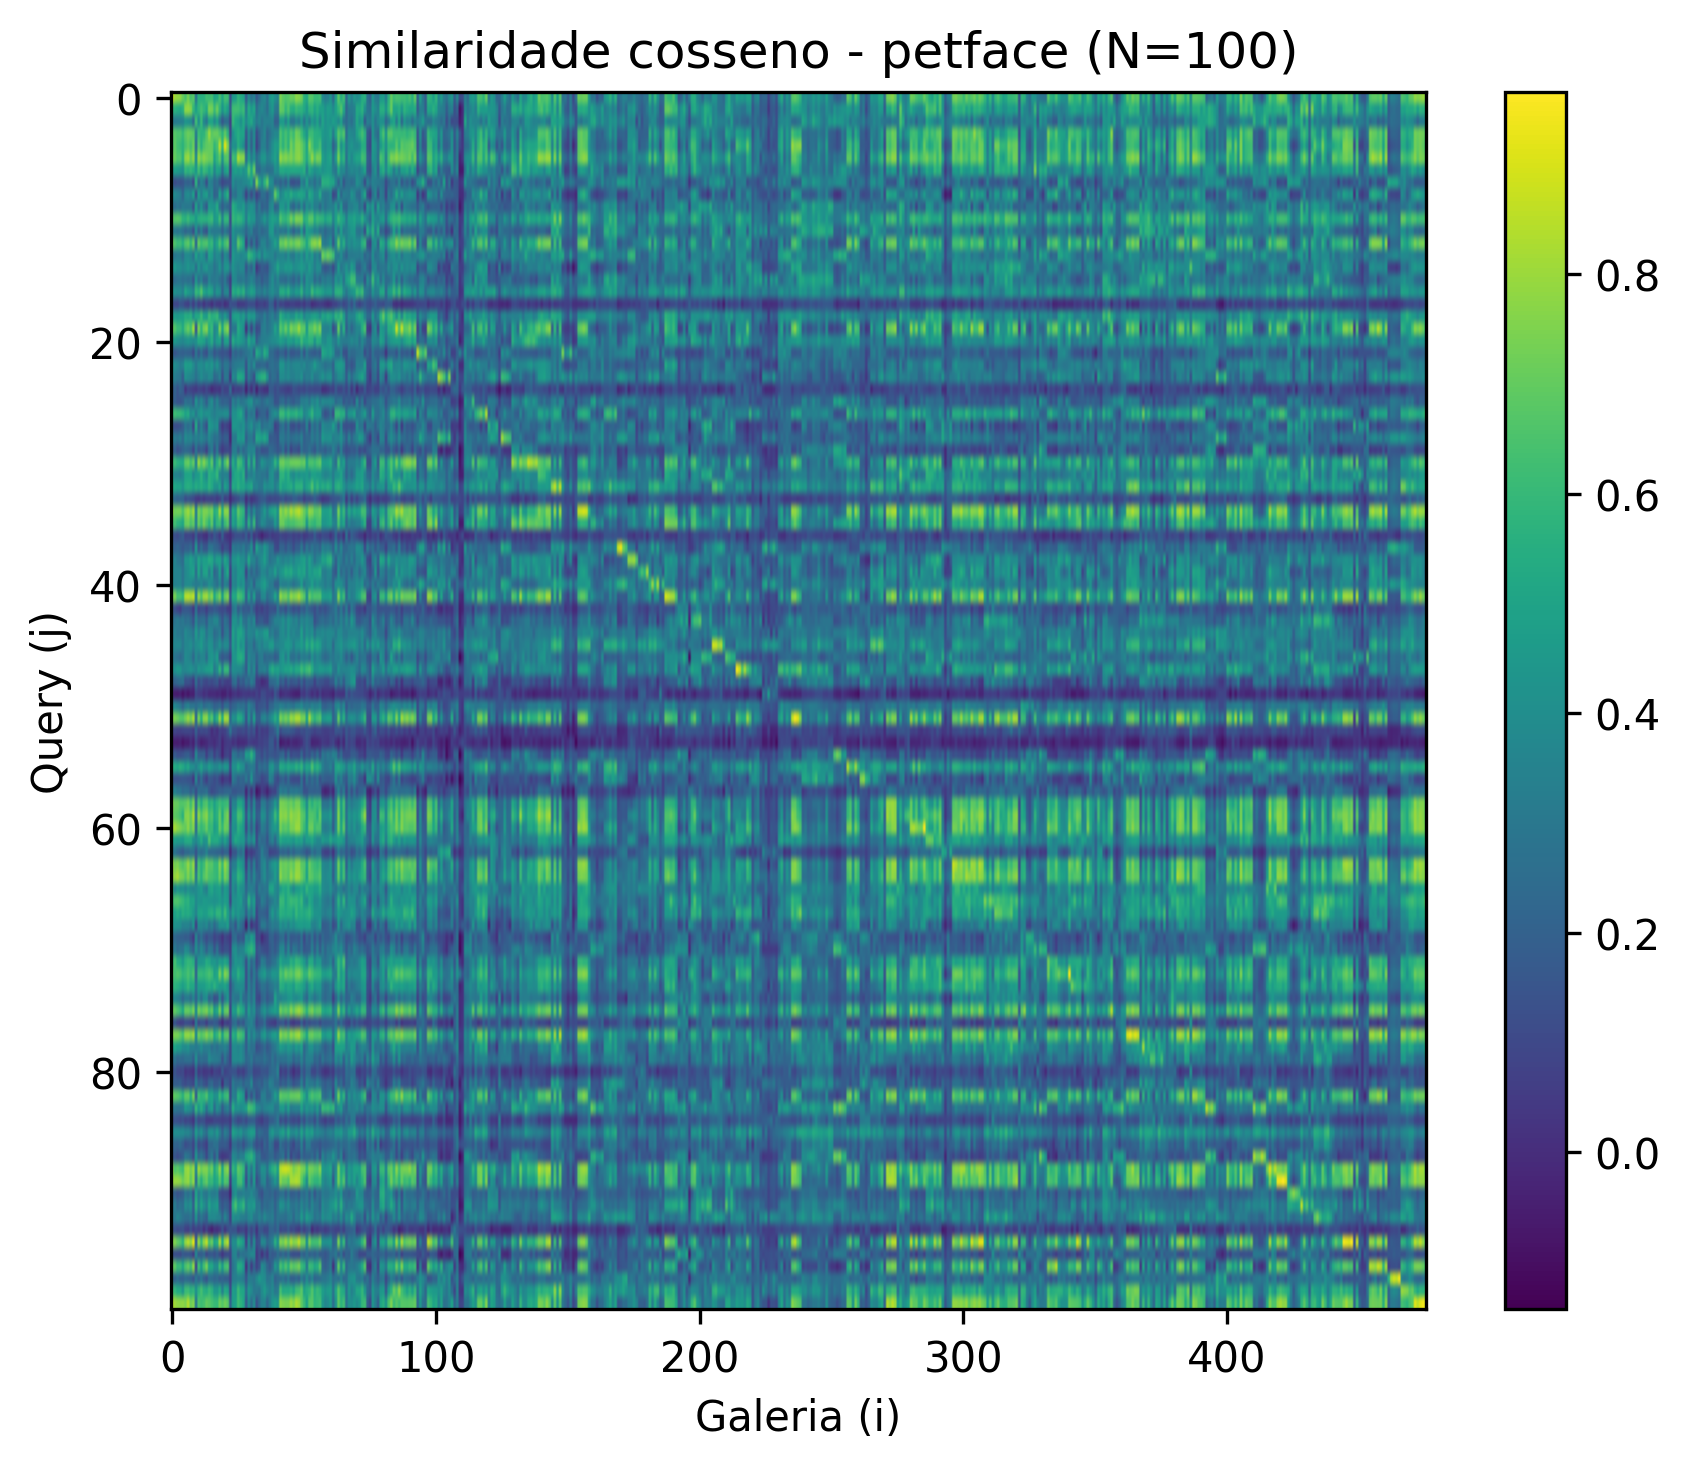
\includegraphics[width=0.80\linewidth]{elementos/figuras/cap5/reid_matriz_sim_n0100.png}
  \fonte{Elaborado pelo autor a partir dos artefatos da run \texttt{dm\_v8}.}
\end{figure}

\begin{figure}[!htb]
  \centering
  \caption[Distribuição de similaridades intra e inter identidades, $N=100$.]{Distribuição de similaridades cosseno entre pares de embeddings classificados como intra-identidade (mesma identidade) e inter-identidades (identidades distintas) no regime closed-set $N=100$.}
  \label{fig:cap5-dist-intra-inter-n100}
  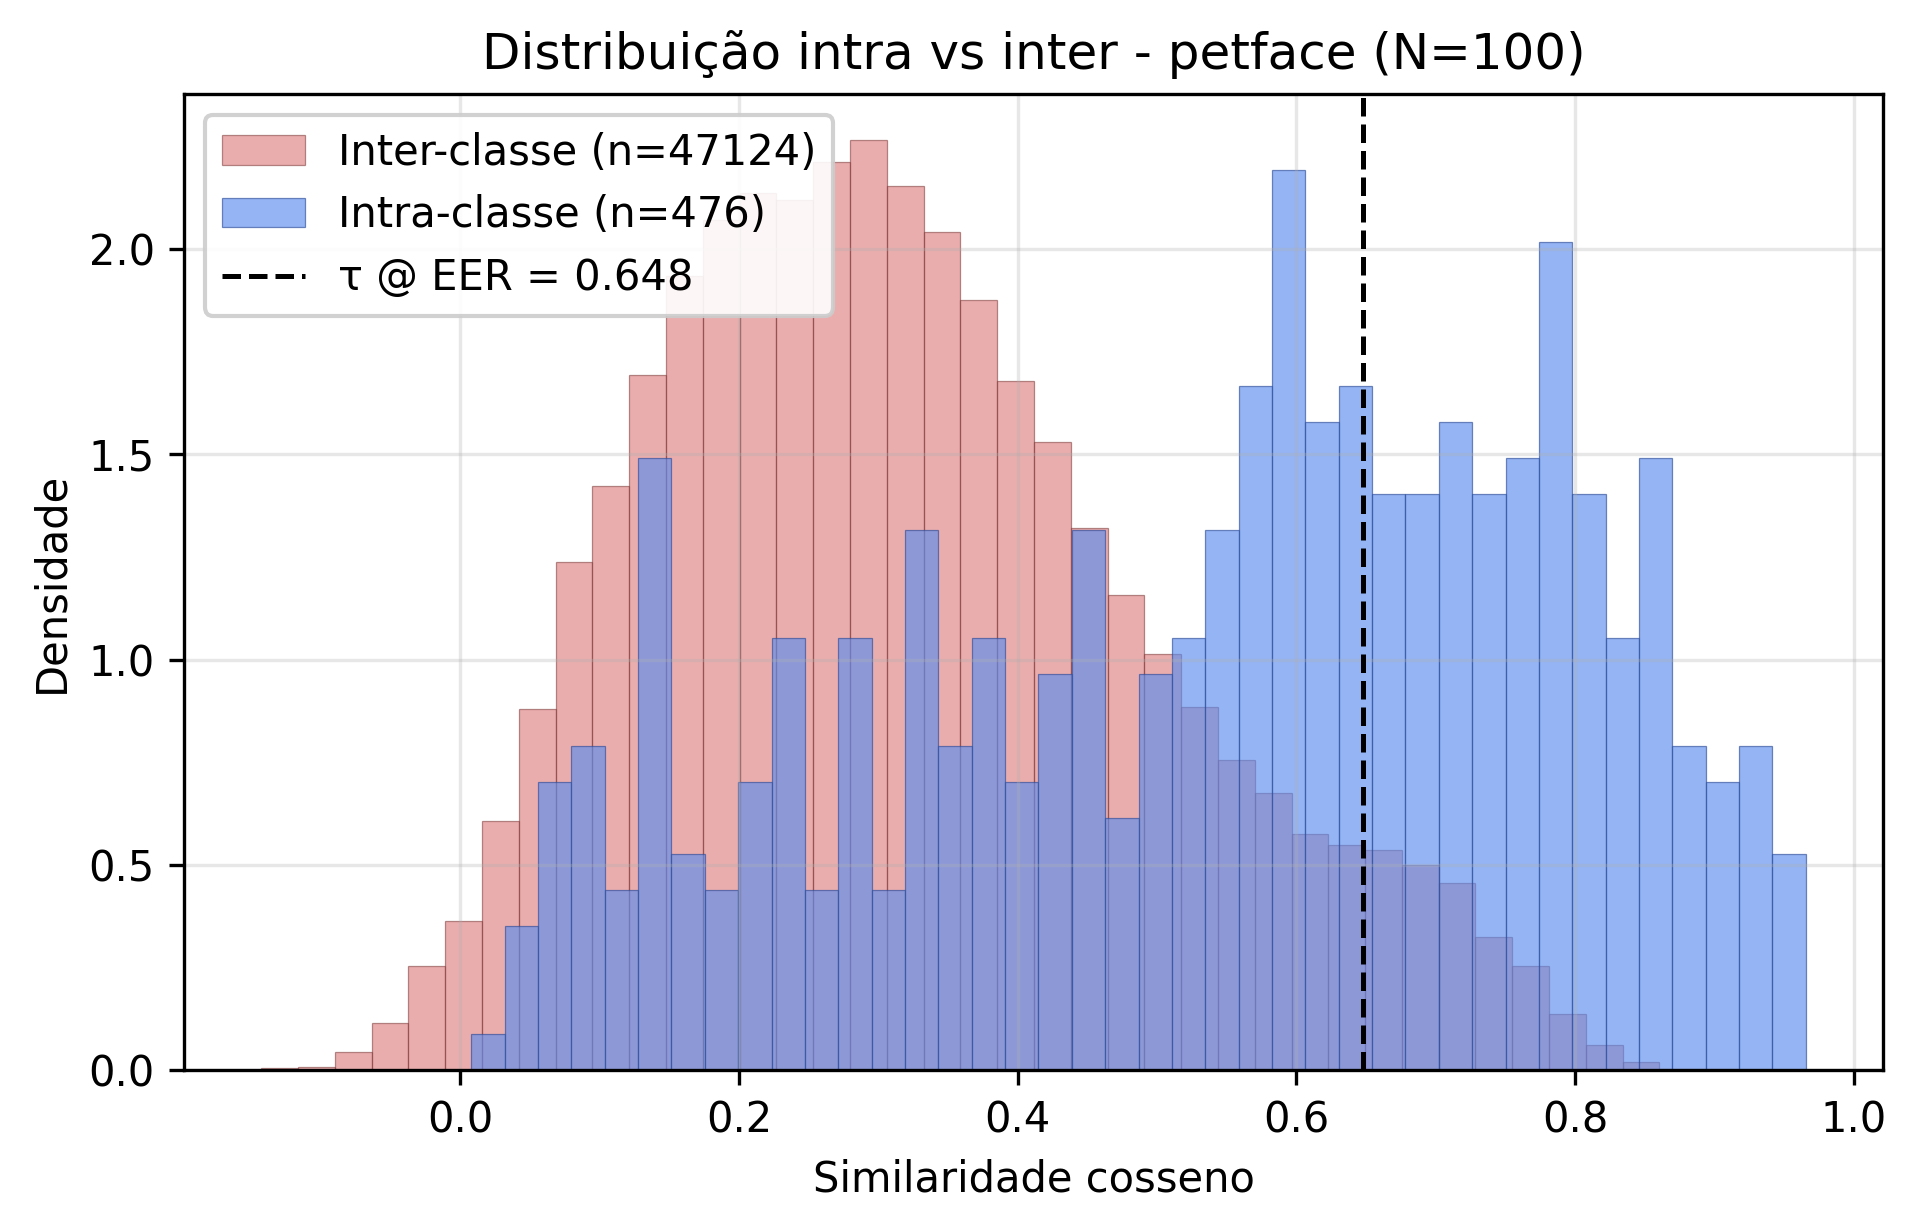
\includegraphics[width=0.80\linewidth]{elementos/figuras/cap5/reid_dist_intra_inter_n0100.png}
  \fonte{Elaborado pelo autor a partir dos artefatos da run \texttt{dm\_v8}.}
\end{figure}

% -------------------------------------------------------------
\section{Fase IV: re-ID em regime open-set}
\label{sec:res-reid-openset}

A extensão para o regime open-set foi conduzida com três sementes aleatórias por escala, recortando consultas em dois grupos (identidades presentes na galeria e identidades ausentes, ou \textit{distractors}), conforme o protocolo descrito no Capítulo~\ref{cap:metodologia}. Os resultados agregados (média e desvio-padrão entre sementes) estão na Tabela~\ref{tab:cap5-reid-openset}, e a curva ROC para cada escala é apresentada na Figura~\ref{fig:cap5-roc-openset}.

\begin{table}[!htb]
  \centering
  \caption[Métricas de re-ID open-set sobre PetFace.]{Métricas de re-ID open-set sobre PetFace, agregadas em três sementes. AUC-ROC mede a separabilidade global entre pares positivos e \textit{distractors}; TPR@FPR fixa o ponto de operação; EER é o limiar onde TPR iguala 1$-$TPR.}
  \label{tab:cap5-reid-openset}
  \begin{tabular}{rcccccc}
    \toprule
    \textbf{N} & \textbf{AUC-ROC ($\mu\pm\sigma$)} & \textbf{TPR@FPR=1\%} & \textbf{TPR@FPR=5\%} & \textbf{EER} & \textbf{Rank-1 open} & \textbf{Sementes} \\
    \midrule
    50  & 0,647 $\pm$ 0,051 & 0,213 & 0,280 & 0,360 & 0,213 & 3 \\
    100 & 0,655 $\pm$ 0,050 & 0,107 & 0,287 & 0,380 & 0,107 & 3 \\
    200 & 0,610 $\pm$ 0,069 & 0,087 & 0,177 & 0,397 & 0,087 & 3 \\
    \bottomrule
  \end{tabular}
  \fonte{Elaborado pelo autor a partir de \texttt{openset\_resumo.csv} (run \texttt{dm\_v8}).}
\end{table}

\begin{figure}[!htb]
  \centering
  \caption[Curvas ROC open-set por escala de catálogo.]{Curvas ROC para a tarefa de re-ID open-set sobre PetFace em três escalas. Cada painel corresponde a uma das escalas $N \in \{50, 100, 200\}$, com a curva média entre sementes.}
  \label{fig:cap5-roc-openset}
  \begin{minipage}{0.32\linewidth}\centering
    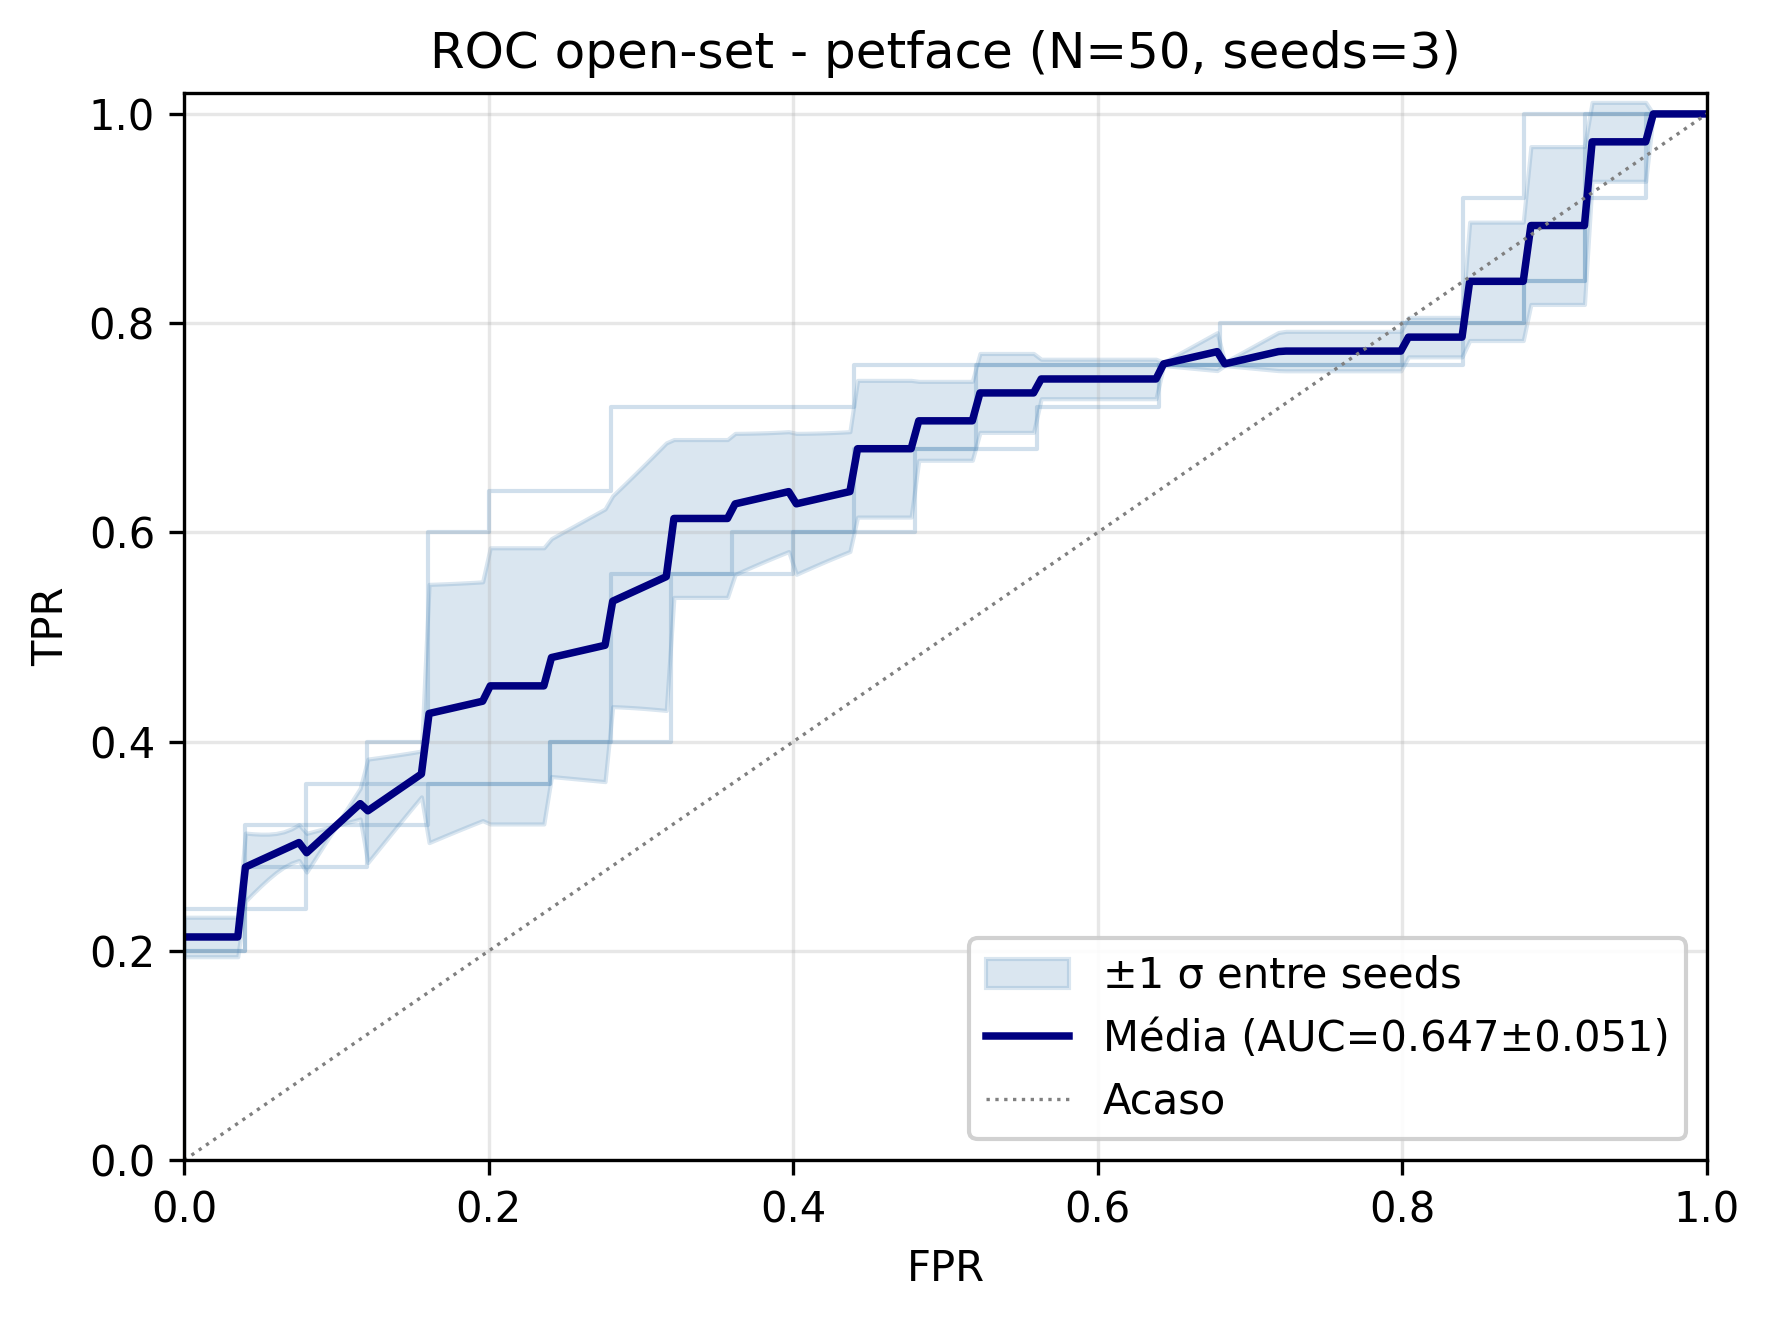
\includegraphics[width=\linewidth]{elementos/figuras/cap5/reid_roc_openset_n0050.png}\\
    \footnotesize (a) $N=50$
  \end{minipage}\hfill
  \begin{minipage}{0.32\linewidth}\centering
    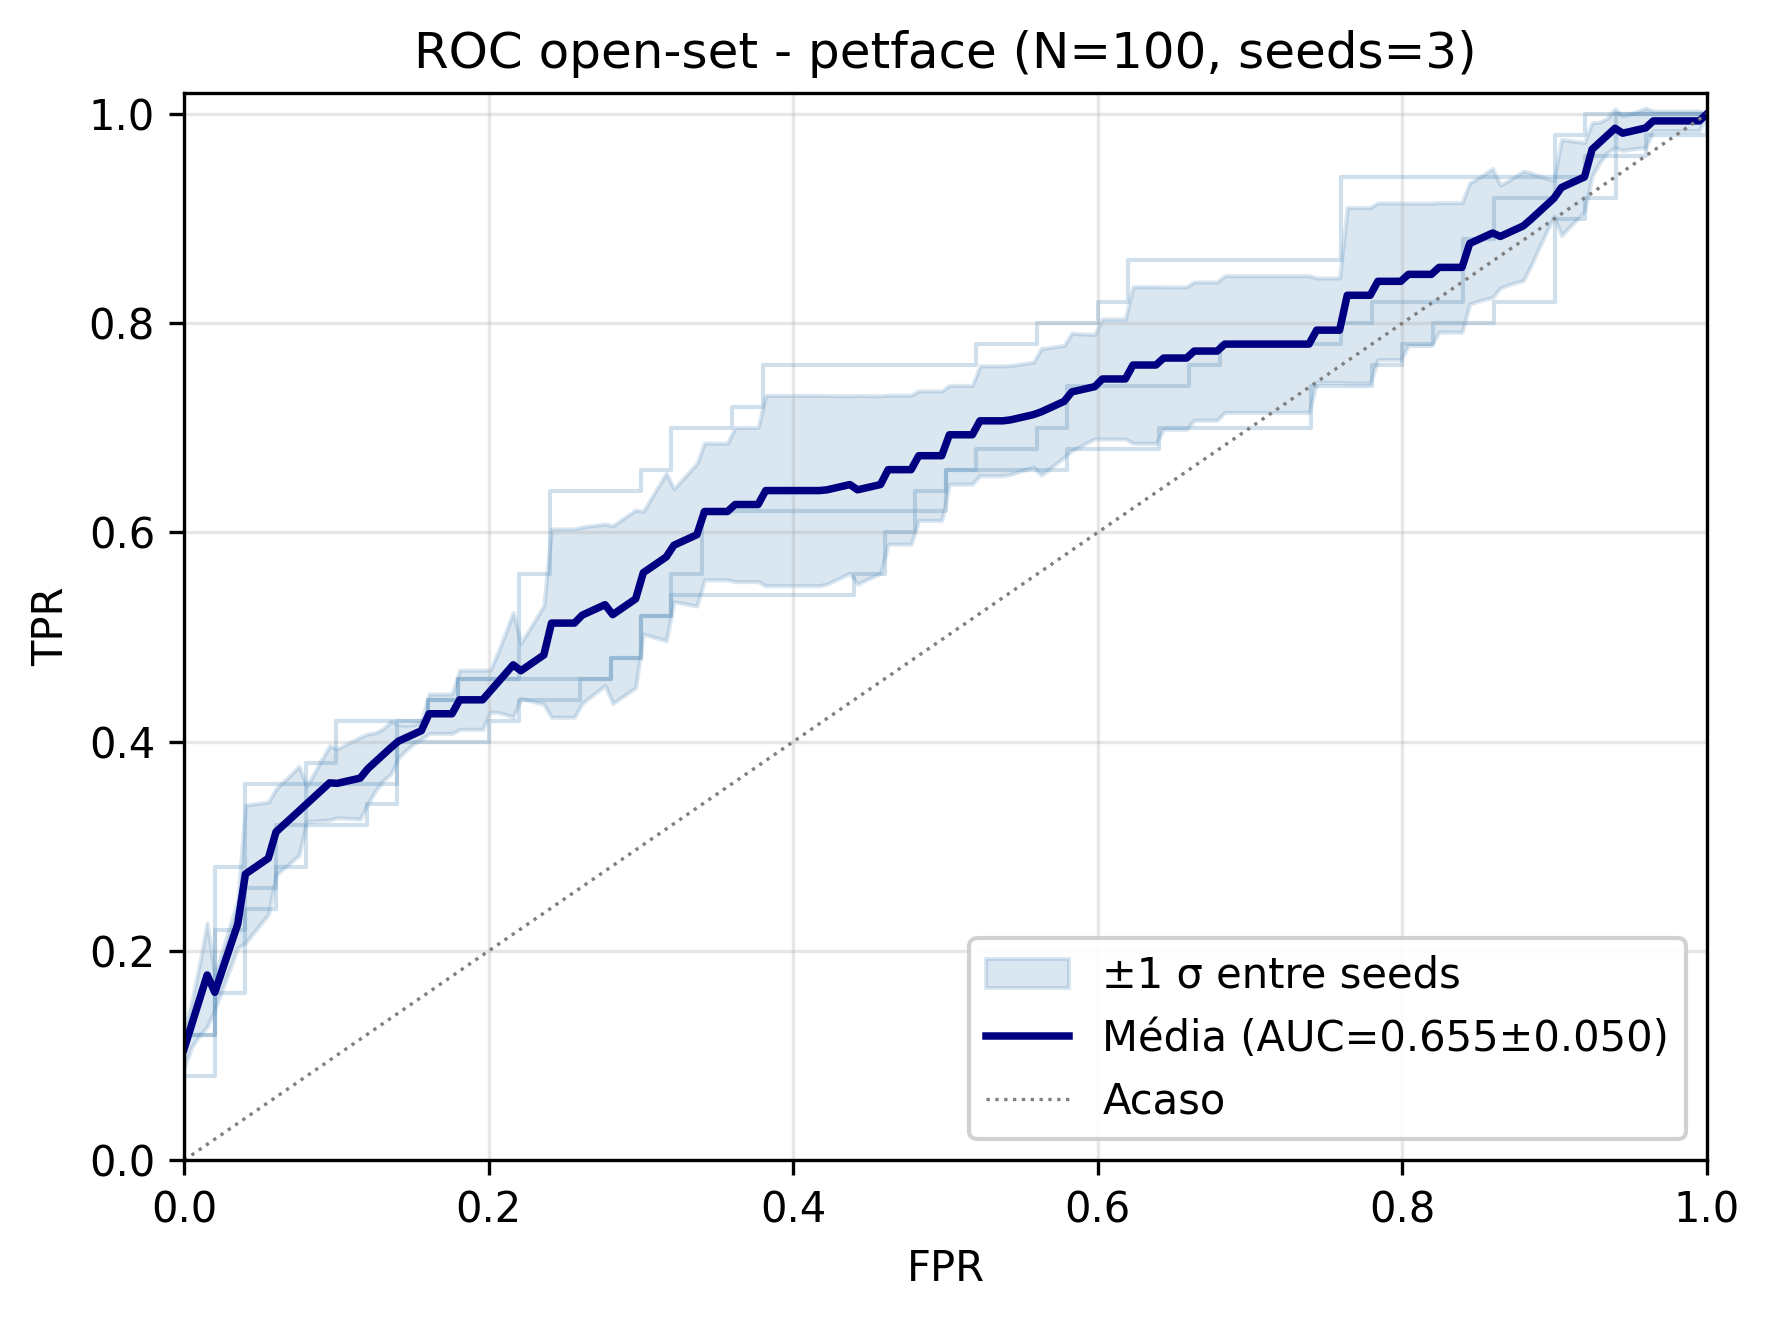
\includegraphics[width=\linewidth]{elementos/figuras/cap5/reid_roc_openset_n0100.png}\\
    \footnotesize (b) $N=100$
  \end{minipage}\hfill
  \begin{minipage}{0.32\linewidth}\centering
    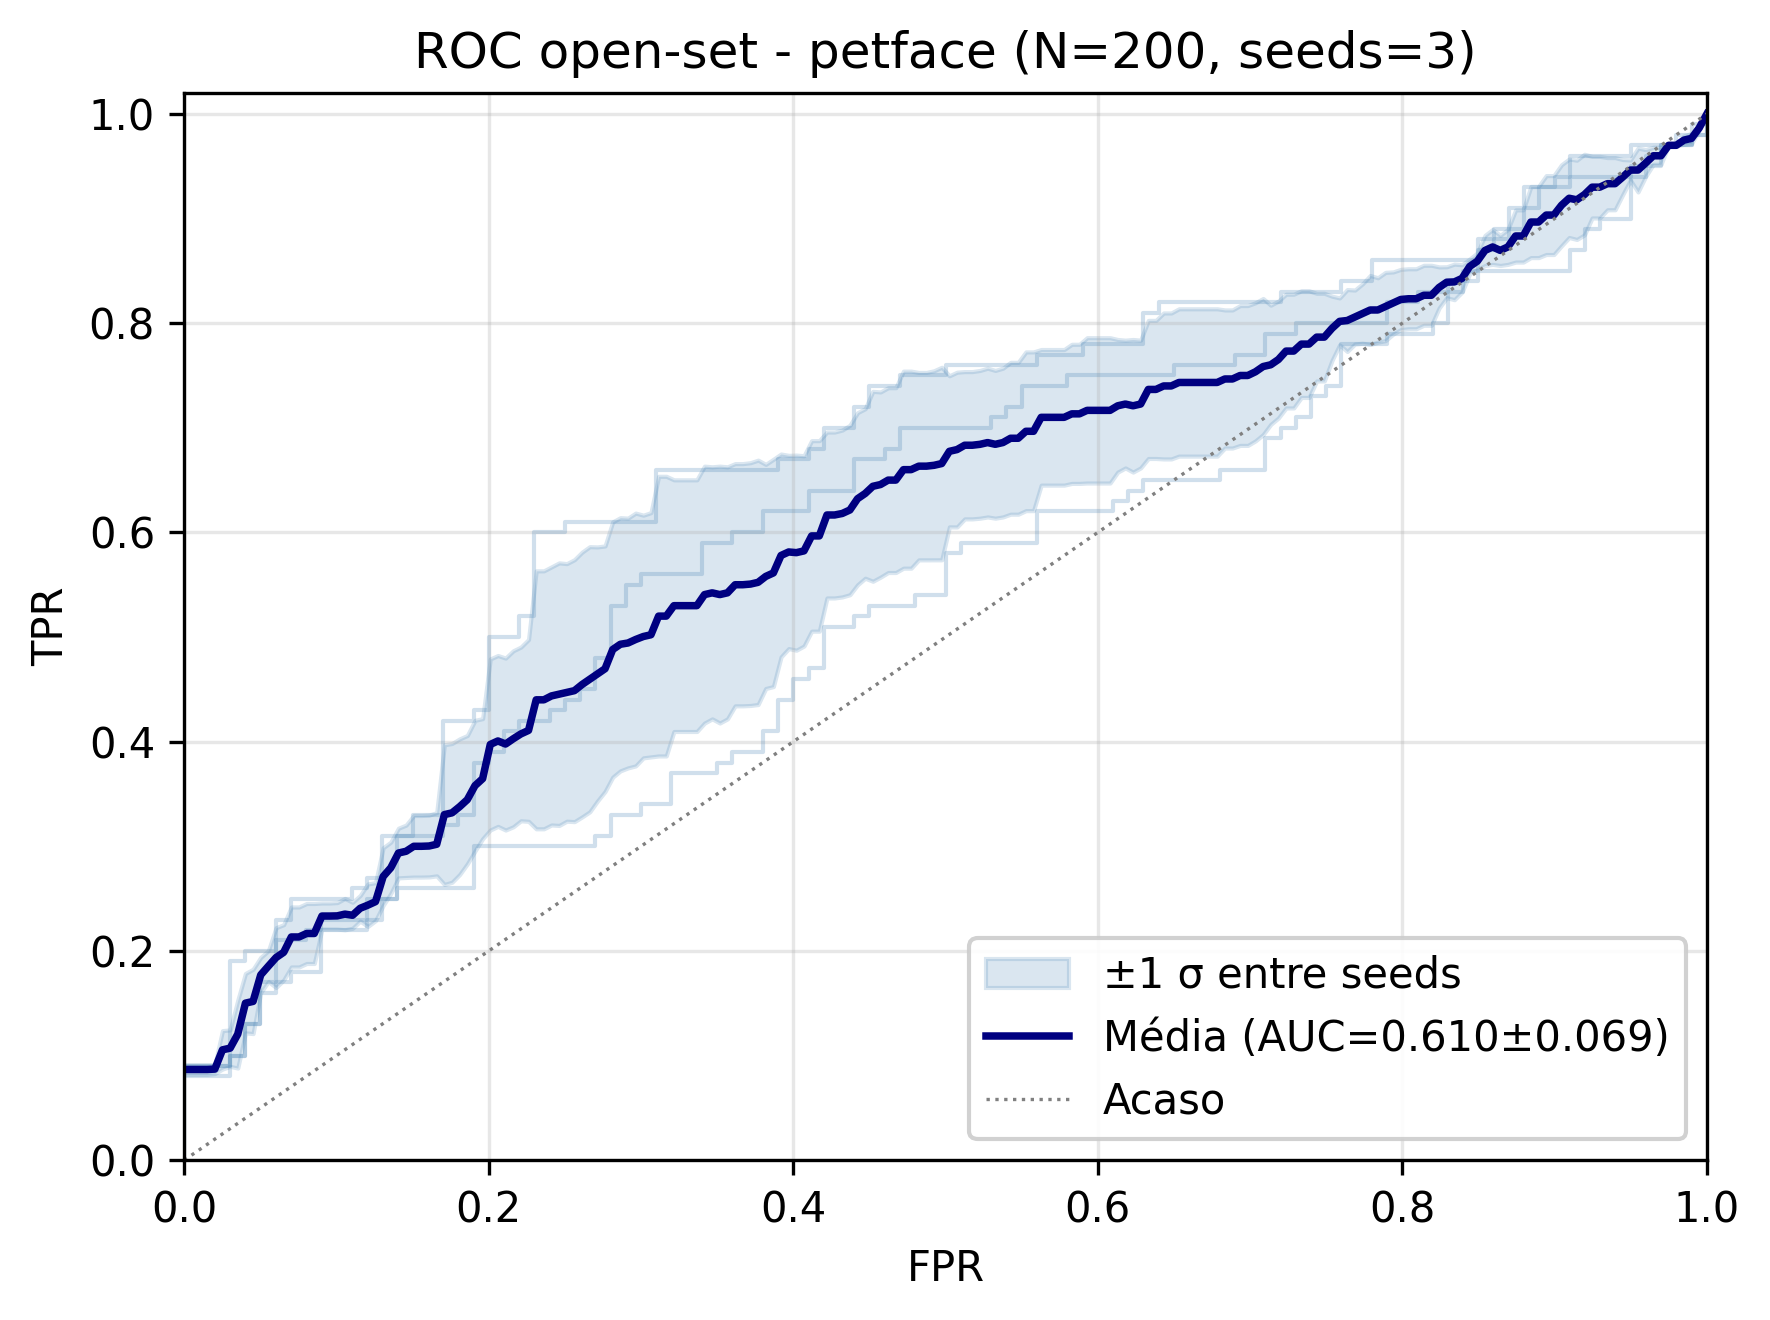
\includegraphics[width=\linewidth]{elementos/figuras/cap5/reid_roc_openset_n0200.png}\\
    \footnotesize (c) $N=200$
  \end{minipage}
  \fonte{Elaborado pelo autor a partir dos artefatos da run \texttt{dm\_v8}.}
\end{figure}

A AUC-ROC oscila em torno de 0,63, com pico em $N=100$ (0,655) e queda em $N=200$ (0,610). O comportamento não-monotônico, com $N=100$ ligeiramente acima de $N=50$, está dentro do desvio-padrão observado (0,050 a 0,069), de modo que a interpretação mais conservadora é a de um patamar próximo, com a degradação real só se manifestando claramente em $N=200$. Os três valores permanecem acima da linha de chance (AUC = 0,5), confirmando que os embeddings de MegaDescriptor retêm sinal discriminativo útil mesmo sem treinamento dirigido à espécie em estudo, mas a margem em relação à chance é modesta e diminui com a escala.

O efeito mais marcante no regime open-set, entretanto, é a queda da métrica TPR a FPR fixo. Em FPR = 1\%, ponto de operação rigoroso característico de sistemas que toleram poucos falsos positivos, a fração de pares positivos corretamente aceitos cai de 0,213 ($N=50$) para 0,107 ($N=100$) e 0,087 ($N=200$). Em FPR = 5\%, regime mais tolerante, os valores são 0,280, 0,287 e 0,177, respectivamente. A leitura combinada é que um limiar fixo, escolhido em uma escala pequena, perde grande parte da sua eficácia quando a galeria cresce: o número de pares negativos aumenta proporcionalmente, e o mesmo limiar passa a aceitar uma fração menor de positivos para manter o mesmo nível de falsos alarmes. A EER, que cresce de 0,360 para 0,397, confirma o mesmo fenômeno: o ponto em que se equilibram falsos positivos e falsos negativos torna-se progressivamente mais alto.

Em termos de Rank-1 open, métrica que combina o ranking closed-set com o veto open-set, o resultado é numericamente igual ao TPR@FPR=1\% nas três escalas. Essa coincidência reflete a maneira como a métrica foi calculada (com um único limiar conservador), e indica que, sob o ponto de operação adotado, o sistema open-set degrada em paralelo às duas dimensões.

% -------------------------------------------------------------
\section{Síntese dos resultados}
\label{sec:res-sintese}

Os números reportados nas seções anteriores sustentam três leituras complementares. A cascata Fases II--III opera de forma coerente nos dois extremos da família Felidae: aceita gatos domésticos com folga (83,4\%) no corpus \texttt{kaggle\_cats} e rejeita felídeos não-domésticos com folga (apenas 0,3\% de aceitação) no Felidae. A diferença entre as taxas de detecção animal (61,3\% contra 97,3\%) reflete não uma falha do detector, mas a natureza distinta dos enquadramentos típicos de cada corpus, com imagens de cativeiro e de campo concentrando o sujeito mais ao centro do quadro. Esse achado é relevante para o desenho operacional do sistema, pois indica que a taxa absoluta de aproveitamento por fonte depende fortemente da estatística de enquadramento da fonte, não apenas da capacidade dos modelos pré-treinados.

A Fase IV closed-set demonstra que o backbone MegaDescriptor, sem ajuste fino para a espécie em estudo, sustenta um Top-1 de 0,720 em galerias pequenas e mantém Top-10 acima de 0,76 nas três escalas testadas. Esse patamar viabiliza o uso assistido do ranking, isto é, fluxos em que o sistema sugere as 10 hipóteses mais prováveis e um operador humano confirma a identidade. A degradação do Top-1 com o aumento de $N$ está dentro do esperado para o backbone, e a estabilização entre $N=100$ e $N=200$ sugere que, a partir de um determinado tamanho, o desempenho passa a ser limitado pela própria capacidade discriminativa do espaço de embeddings, e não pelo crescimento marginal da galeria.

A Fase IV open-set é o cenário em que o sistema enfrenta sua maior limitação observada. Embora as AUC-ROC permaneçam acima da chance, a queda da TPR a FPR fixo, de 0,213 em $N=50$ para 0,087 em $N=200$ no ponto de operação rigoroso, mostra que limiares estabelecidos em escalas pequenas não se transferem diretamente para catálogos maiores. Esse achado tem consequência direta para o projeto da Felinet: a operação em campo em uma colônia de gatos da AEX Gatos do C2, ou em colônias semelhantes em pontos de alimentação universitários, exigirá calibração específica do limiar de aceitação por escala, bem como mecanismos de revisão humana para os casos em que o ranking automático apresentar similaridade próxima ao limiar de decisão.

A leitura conjunta dos três blocos (cascata operacional, re-ID closed-set e re-ID open-set) aponta para um sistema funcional dentro do recorte experimental adotado, com limites bem caracterizados em cada fase. As implicações dessa caracterização para a operação em campo, as limitações remanescentes e o conjunto de trabalhos futuros que dela decorrem são tratadas no Capítulo~\ref{cap:conclusao}.
